\section{Что мы измерили до того, как что-то строить}

Первое, что было сделано --- простая базовая линия и разбор, почему она ведёт себя так, как ведёт.
Без этого нет способа отличить работающую конструкцию от красивой.

Базовая линия: счётчики фрагментов Моргана радиуса 2 (2048 бит), 217 дескрипторов RDKit, градиентный
бустинг, пятикратная кросс-валидация по кластерам Бутины при пороге сходства 0.35.

\begin{figure}[htbp]\centering
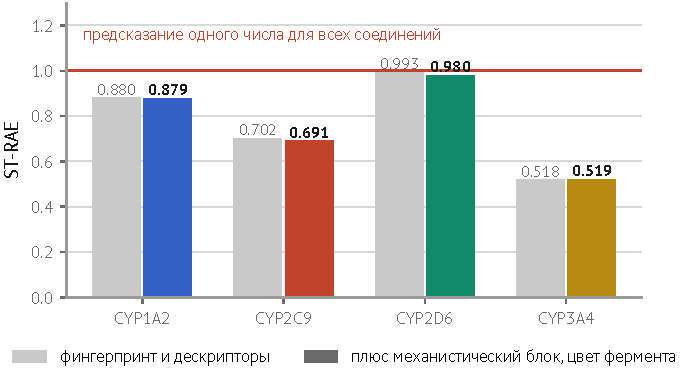
\includegraphics{fig/baseline}
\caption{Базовая линия регрессионного трека. Красная линия --- уровень предсказания одного числа
для всех соединений. CYP3A4 предсказывается вдвое лучше этого уровня, CYP2D6 --- на две сотых.}
\label{fig:baseline}
\end{figure}

Числа по ферментам: 1A2 --- ST-RAE 0.880 при Спирмене 0.497; 2C9 --- 0.702 и 0.583; 2D6 --- 0.993
и 0.351; 3A4 --- 0.518 и 0.764. Макро 0.773. Коэффициент детерминации на тех же фолдах: 0.216, 0.350,
0.122, 0.589.

CYP2D6 практически не предсказывается. Это и стало главным предметом разбирательства, потому что от
объяснения зависит, что вообще строить дальше.

\subsection{Версия первая: метки шумные, учить нечего}

Если почти весь разброс опубликованных активностей --- погрешность измерения, то потолок для любой модели
низкий и делать нечего. Обычно разделить настоящий разброс и шум трудно, но здесь вместе с каждым значением
опубликована его собственная стандартная ошибка.

Дисперсии независимых источников разброса складываются, поэтому
\begin{equation}
\Var(\text{наблюдаемое}) = \Var(\text{настоящее}) + \Var(\text{шум}),
\qquad
\text{надёжность} = 1 - \frac{\Var(\text{шум})}{\Var(\text{набл.})} .
\label{eq:rel}
\end{equation}

Надёжность --- доля разброса меток, которая приходится на настоящие химические различия. Она же задаёт
потолок $R^2$ для любой модели на этих метках: предсказать шум нельзя.

Для CYP2D6 стандартное отклонение меток 0.916, среднеквадратичная погрешность одного измерения 0.236,
надёжность 0.934. По остальным ферментам от 0.898 до 0.948. Версия не подтвердилась: сигнала в метках
достаточно. Сравнивая достигнутый $R^2$ с этим потолком, модель осваивает на 2D6 лишь восьмую часть
доступного ($0.122$ из $0.934$) и две трети на 3A4 ($0.589$ из $0.898$).

Оговорка, которую надо держать в голове. Слово «среднеквадратичная» здесь существенно: медианная
погрешность на 2D6 равна 0.069, то есть в три с половиной раза меньше, а почти шестьдесят процентов всей
шумовой дисперсии дают верхние пять процентов соединений с развалившейся подгонкой. В разложение
\eqref{eq:rel} идёт именно средний квадрат, так что число верное, но шум резко гетероскедастичен,
и взвешивание по индивидуальной погрешности важнее, чем кажется по среднему.

\subsection{Версия вторая: не хватает нужных признаков}

Как разобрано в разделе~\ref{sec:isoforms}, CYP2D6 узнаёт субстраты через солевой мостик
с протонированным азотом, а не через общую липофильность. Фингерпринт про заряд не знает: третичный амин
и амид для него --- два похожих азота в похожем окружении, хотя доля заряженной формы у них различается
в сотни раз.

Собрали блок из 28 химически осмысленных чисел: оценка $\mathrm{p}K_a$ самого основного центра, доля
протонированной формы при pH 7.4, полный заряд молекулы, счётчики классов азота и кислотных групп,
топологическое расстояние от заряженного азота до ближайшего ароматического кольца. Оценщик
$\mathrm{p}K_a$ --- правило: базовое значение класса минус индуктивный штраф от электроноакцепторных
заместителей с затуханием по числу связей. На двадцати соединениях с литературными значениями средняя
ошибка 0.60 единицы, медианная 0.2, и на бинарный вопрос «заряжено ли при 7.4» правило ответило верно
во всех двадцати случаях.

Результат двойственный, и это тот случай, когда полезно смотреть на две метрики сразу.

По ST-RAE выигрыша нет. Парный бутстрап по соединениям даёт для 2D6 разность $-0.012$ с интервалом
от $-0.041$ до $+0.017$; на макро-уровне $-0.0056$ с интервалом от $-0.0155$ до $+0.0041$. Интервалы
накрывают ноль.

По ранжированию выигрыш есть, и он избирателен именно так, как предсказывает химия. Спирмен на 2D6 растёт
с 0.351 до 0.403, разность $+0.052$ с интервалом от $+0.022$ до $+0.082$ и вероятностью отсутствия
прироста 0.001. На 2C9 $+0.014$ на грани значимости, на 1A2 и 3A4 нули с интервалами шириной в две сотых.

Ещё показательнее вот что: модель, построенная только на двадцати восьми механистических числах, без
фингерпринта и дескрипторов, воспроизводит на 2D6 92 процента ранжирующей способности модели на
фингерпринте с дескрипторами и 80 процентов от полной модели со всеми блоками --- против 43--53 процентов
на трёх остальных при любом из двух знаменателей. Сигнал CYP2D6 низкоразмерный и химически специфичный.

Итог: механизм назван верно, но выигрыш по метрике соревнования неотличим от нуля. Признаки --- часть
ответа, не главная его часть.

\subsection{Версия третья: дело в том, какие соединения попали в выборку}
\label{sec:d6}

\begin{figure}[htbp]\centering
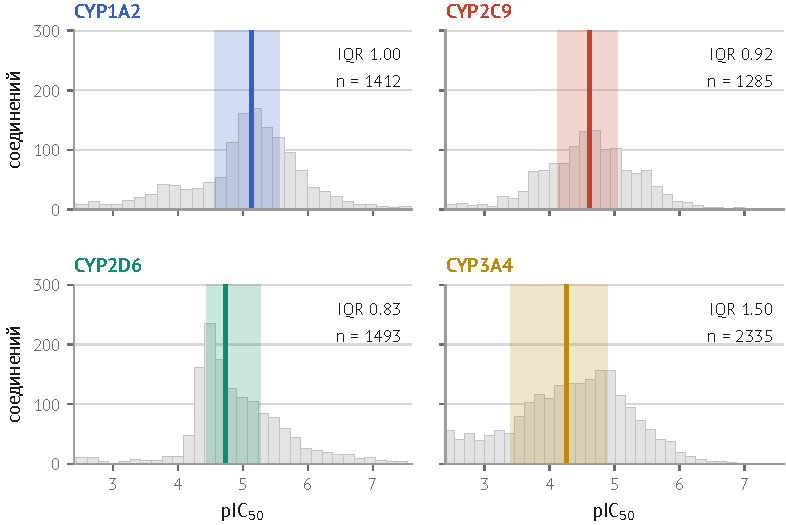
\includegraphics{fig/dists}
\caption{Распределения измеренных активностей. Цветом выделены средние 50 процентов соединений.
У CYP3A4 задача во многом сводится к тому, чтобы отделить левую часть от правой. У CYP2D6 левой части
почти нет, и модели приходится различать соединения внутри узкой полосы.}
\label{fig:dists}
\end{figure}

У CYP2D6 отбор оставил узкую полосу: средняя половина соединений уместилась в интервал шириной 0.83
логарифмической единицы против 1.50 у CYP3A4. Это ограничение диапазона, оно же selection
on the dependent variable: если отобрать объекты по интересующему признаку и потом мерить связь только
среди отобранных, связь ослабевает, хотя в полной популяции она никуда не делась.

Проверка требует второго показателя активности того же фермента, измеренного \emph{без} отбора. Он есть:
$\log_2$fc скрининга, снятый для 4375 соединений подряд, включая неактивные. Учим ту же модель на тех же
признаках и тех же фолдах предсказывать его вместо $\pic$.

Чтобы это не превратилось в сравнение «больше примеров против меньше», сделан контроль: из соединений
со скринингом случайно выбирается ровно столько же, сколько у этого фермента меток кривых.

\begin{figure}[htbp]\centering
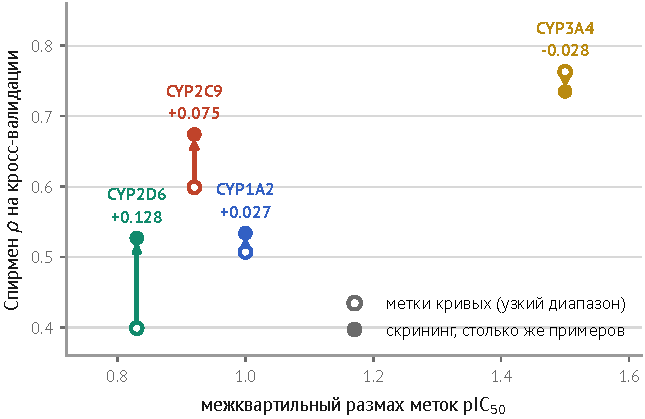
\includegraphics{fig/range}
\caption{Выигрыш от перехода на показатель с полным диапазоном против ширины полосы меток. Пустой кружок ---
качество на метках кривых, закрашенный --- на скрининге при равном числе обучающих примеров. Стрелка
тем длиннее, чем уже полоса меток, и на CYP3A4 разворачивается.}
\label{fig:range}
\end{figure}

Прирост монотонно падает с ростом размаха меток: 2D6 $+0.128$, 2C9 $+0.075$, 1A2 $+0.027$, 3A4 $-0.028$.
Четыре точки, монотонно, и отрицательный знак на CYP3A4 работает внутренним контролем против объяснения
«скрининг просто легче предсказуем сам по себе». На 2D6 при равном числе примеров $R^2$ поднимается
с 0.136 до 0.323.

Модель прекрасно умеет учить химию CYP2D6, но не может показать это на выданных метках. Основная причина
провала --- геометрия меток, и чинится она не признаками, а тем, что в правдоподобие входит источник
с полным диапазоном. На этом и построено всё остальное.

Честная оговорка про контроль: выровнено количество примеров, но не форма распределения меток. Совсем
чистый эксперимент требует подобрать подвыборку так, чтобы совпадало и то и другое.
